\documentclass[main.tex]{subfiles}
\begin{document}
\chapter{動態規劃}

\section{輪廓線DP}
\par 輪廓線DP是位元DP的一種變形。通常用來解決一些 2D 表格上面的問題。直接來看一個經典的題目:
\problem{\href{https://cses.fi/problemset/task/2181/}{Counting Tilings (CSES 2181)}}{
在一個\(n \times m\)表格上用\(1 \times 2\)的骨牌填滿(可以直放或橫放),骨牌不能重疊,有幾種方法?輸出模\(10^9 + 7\)的結果。

$1\leq n \leq 10, 1 \leq m \leq 1000$
}

如果有學好前面位元DP的話,應該可以想到這樣的一個作法:令$dp[i][s]$代表目前在第$i$列 ($i \leq m$),填滿的格子用 bitmask $s$表示,並且$0$到$i-1$列之前全部填滿,$i+1$列之後全部沒有填的方法數。我們可以枚舉所有填滿$s$的方法,並且轉移到相對應的狀態。小心實做的話,這樣的複雜度會是$O(m3^n)$或是更好($O(Fib_{2n} m)$,$Fib_n$為費式數列第$n$項),對於這題來講已經可以通過了,不過以下還是解釋另一個方法。
\par 可以發現,每次放一片骨牌只會影響到周圍的狀態,那如果可以在轉移的時候只放一片的話就能少考慮很多東西! 這個時候就能引入輪廓線的概念:
\smallskip
\begin{center}
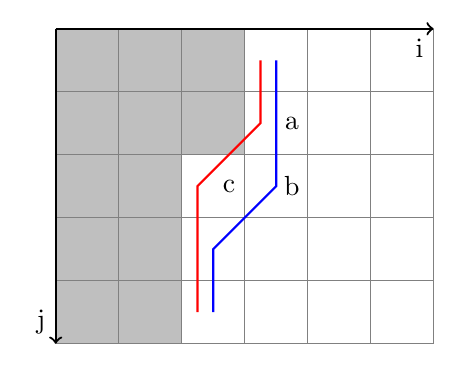
\begin{tikzpicture}
\fill[lightgray] (0,0) rectangle (1.6,4);
\fill[lightgray] (0,2.4) rectangle (2.4,4);
\draw[step=0.8cm,gray,very thin] (0,0) grid (4.8, 4);
\draw[red, thick] (2.6, 3.6) -- (2.6, 2.8) -- (1.8, 2.0) -- (1.8, 0.4);
\draw[blue, thick] (2.8, 3.6) -- (2.8, 2.0) -- (2.0, 1.2) -- (2.0, 0.4);
\node[draw=none] at (3.0, 2.8){a}; 
\node[draw=none] at (3.0, 2.0){b}; 
\node[draw=none] at (2.2, 2.0){c}; 
\draw[thick,->] (0,4) -- (0,0) node[anchor=south east] {j};
\draw[thick,->] (0,4) -- (4.8,4) node [anchor=north east]{i};
\end{tikzpicture}
\end{center}
\par (註:這裡的 dp 都是 0-base)令$dp[i][j][s]$代表目前已填滿$0$到$i-1$列以及第$i$列的$0$到$j-1$項,且目前的輪廓線上格子填滿的狀態是$s$的方法數。這裡的輪廓線是指第$i+1$列的$0$到$j-1$項以及第$i$列的$j$到$n-1$項共$n$格。用上圖來看的話,目前算好了$dp[3][1]$,那灰色格子都被填滿,紅色(左邊)線段為$s$表示的輪廓線,而我們要算$dp[3][2]$,把輪廓線更新成藍色線段。現在來考慮轉移的方式:
\begin{itemize}
    \item 用一個骨牌填滿$c, b$,那原本$c$是空的
    \item 用一個骨牌填滿$a, b$,那$a$是空的,$c$必須是滿的
    \item 不用骨牌填滿$b$,那$c$必須是滿的
\end{itemize}
\par 這裡的重點就是只考慮$b$要如何填滿,而由前面的分析可以發現,只需要$dp[i][j-1]$裡的狀態就能更新$dp[i][j]$,因此我們可以使用滾動 dp 簡化實作,可以用下面的程式碼加強理解。
\begin{C++}
#define mod 1000000007
int dp[2][1<<10];
void madd(int &u, int v) { //u = (u + v) % mod
	u += v - mod; u += mod & (u>>31);
}
int main() {
	int n, m;
	cin >> n >> m;
	dp[0][(1<<n) - 1] = 1;
	for (int i = 0;i < m;i++) {
		for (int j = 0;j < n;j++) {
			for (int s = 0;s < (1<<n);s++) {
			    if (!(s & (1<<j))) madd(dp[1][s ^ (1<<j)], dp[0][s]); //case 1
				if (j && (s & (1<<j)) && (s & (1<<(j-1)))) {
					madd(dp[1][s], dp[0][s ^ (1<<(j-1))]);
				} //case 2
				if (s & (1<<j)) madd(dp[1][s ^ (1<<j)], dp[0][s]); //case 3
			}
			for (int s = 0;s < (1<<n);s++) {
				dp[0][s] = dp[1][s];
				dp[1][s] = 0;
			}
		}
	}
	cout << dp[0][(1<<n) - 1] << "\n";
}
\end{C++}
\section{例題}
\problem{\href{https://tioj.ck.tp.edu.tw/problems/2153}{開窗戶 (TIOJ 2153)}}{
對於一個$n \times m$的 01 表格,如果每個$2 \times 2$的子矩形(連續)都至少有兩個 1,那麼這個表格是好的。輸出好的表格數模$K$。

$n, m \leq 16, 2\leq K \leq 10^9 + 9$
}
\end{document}
